% ------------------------------------------------------------------------
% -*-TeX-*- -*-Hard-*- Smart Wrapping
% ------------------------------------------------------------------------
\def\baselinestretch{1}

\chapter{Implementation and Testing}
This chapter describes the detailed implementation and testing for my dissertation project.

\section{Implementation}
The main web portal is implemented using incremental approach. The main web portal and forum is built on Django app and the chatbot is built on Flask app. Finally, chatbot is integrated into web portal using cross-origin  resource sharing (CORS).

\subsection{Chatbot Development}

\subsubsection{Libraries and Packages}
The following is a list of the necessary Python packages.
\begin{enumerate}[label=\arabic*.]
	\item tensorflow==2.3.1
	\item nltk==3.5
	\item colorama==0.4.3
	\item numpy==1.18.5
	\item scikit\_learn==0.23.2
	\item Flask==1.1.2
\end{enumerate}

After that, importing all of the required library files are done. There are several libraries, such as:
\begin{enumerate}[label=$\ast$]
	\item nltk (Natural Language Toolkit), that provides many instruments for enhancing text and making it suitable for deep learning algorithms.
	\item json, is a Python module that loads json files straight into the language.
	\item pickle, is an application that loads pickle files.
	\item numpy, which is able to carry out operations in linear algebra in a highly efficient manner.
	\item keras, is the name of the framework for deep learning that can be utilised for training model.
\end{enumerate} 

\subsubsection{Initializing Chatbot Training}
At this point, it is time to begin the process of initialising all of the lists that will be used to hold my natural language data. There is the JSON file that I described previously, which is where the "intents" are stored. The following Figure \ref{fig:9} is a sample of what a typical JSON file truly looks like in its entirety:
\begin{figure}[!h]
	\centering
	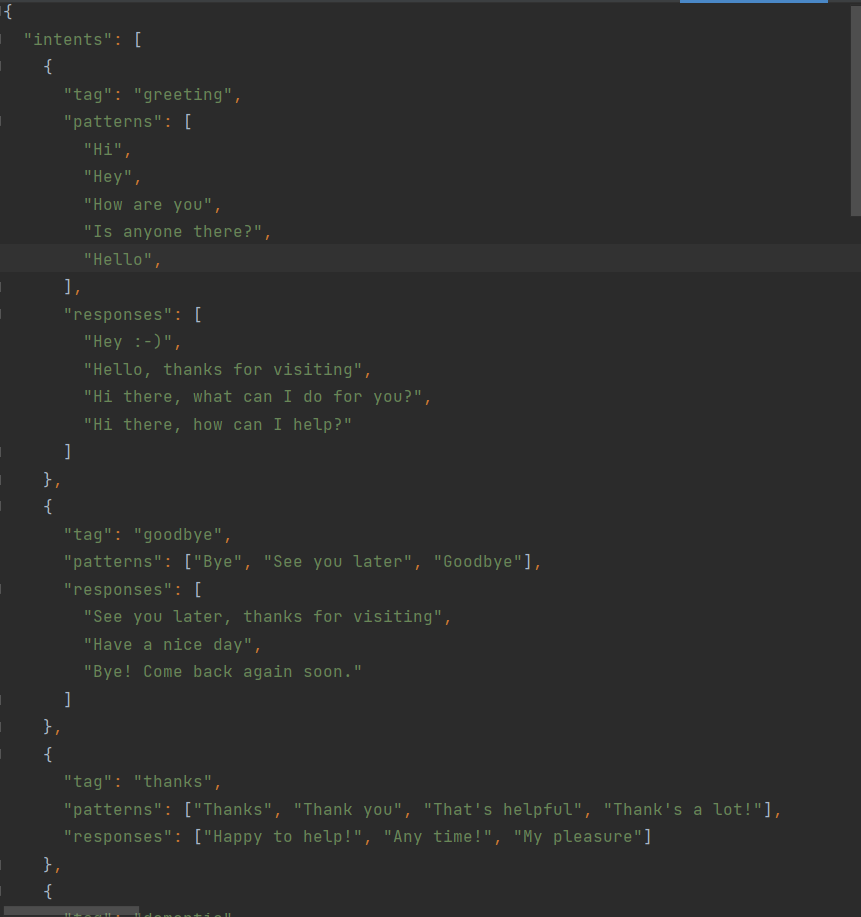
\includegraphics[width=0.8\textwidth]{intent}
	\caption{Simple JSON format.}
	\label{fig:9}
\end{figure}

To load the file, I make use of the json module, and then I store the loaded data to the variable intentions. There are sub-objects included inside the objects themselves. For instance, "patterns" is a property that falls within the category of "intents." Therefore, in order to extract all of the words included inside "patterns," I make use of a nested for loop to do so, and then I add those words to my list of words. The next thing I do is add each pair of patterns to my documents list inside the tag that corresponds to them. I also put the tags into the classes list, and to prevent them from being repeated, I utilise a simple conditional expression.

After that, I take the list of terms and lowercase and lemmatize all of the words that are included inside it. In the event that you were unaware, "lemmatize" is the process of reducing a word to its essential meaning, also known as its lemma. For instance, the phrases "walking," "walked," and "walks" all derive from the base word "walk," which is simply referred to as "walk." Lemmatizing the language serves the objective of reducing everything to the most fundamental level it can possibly be reduced to. When I really analyse these phrases for machine learning, it'll save a lot of time and save me from making errors that aren't essential. This is somewhat similar to the process of stemming, which involves reducing a conjugated word down itself to base form, also known as the root form.

\subsubsection{Building the Deep Learning Model}
Let's set up a training data variable and fill it with some sample information. For each document, I am creating a large nested list with sacks of words within. The output row feature I have only serves as a key to the collection. Next, I do a train-test-split with the patterns serving as the X value and the intentions serving as the Y variable. Now that both our training and test data are prepared, we can go on to the next step of using a deep-learning model from keras that is called Sequential. The following Figure \ref{fig:10} describes the architecture of the model.

\begin{figure}[!h]
	\centering
	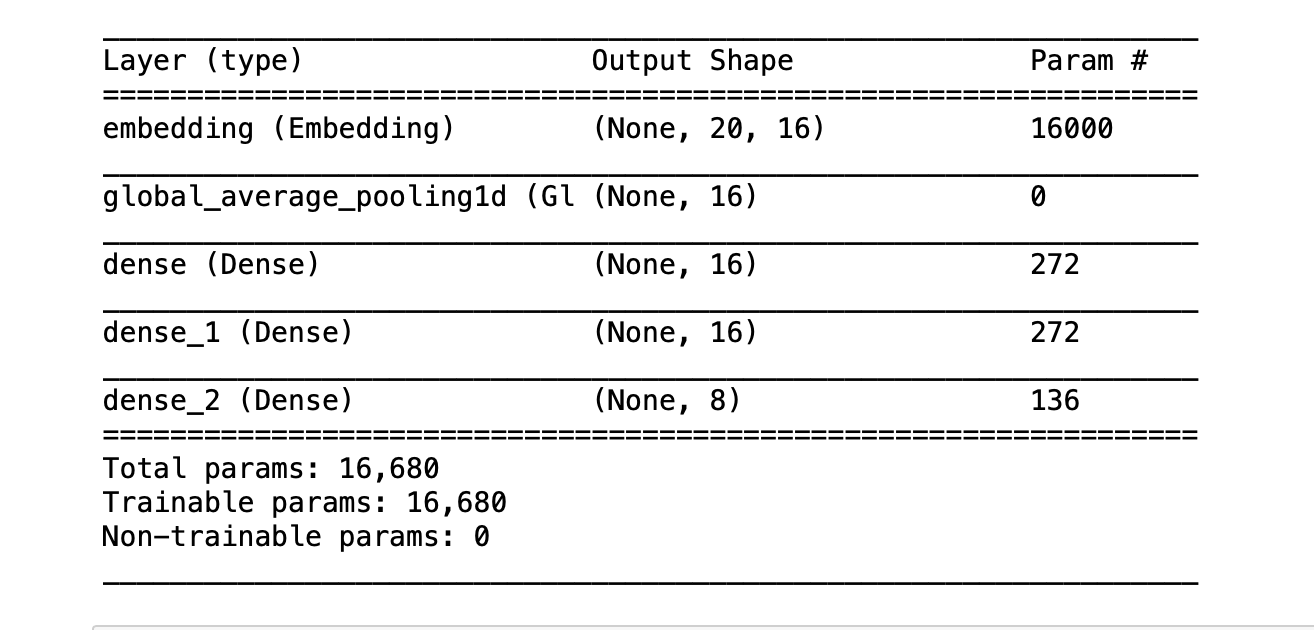
\includegraphics[width=\textwidth]{deeplearning}
	\caption{Sequential Model architecture.}
	\label{fig:10}
\end{figure}

A multi-layer perceptron is one of the simplest types of neural networks, and the Sequential model in keras implements this kind of network. The specific network in question is composed of three layers, the first of which has 128 neurons, the second of which contains 64 neurons, and the third of which contains the same quantity of intents as the amount of neurons. Keep in mind that the purpose of this network is to develop the ability to choose which intent to select given a set of inputs. Stochastic gradient descent, another very hard subject, will be used to train the model in order to improve its accuracy. When compared to traditional gradient descent, stochastic gradient descent performs more effectively. After the training of the model is complete, the whole thing is converted into a numpy array and the file is named chatbot model.h5.

\subsection{Website \& Forum Development}
The Table \ref{table:3} offers a convenient reference for the essential commands that need to run in order to begin the Django development process. Table \ref{table:4} on Appendix lists all the required dependencies for the website development.
\begin{table}[!h]
	\centering
	\begin{tabular}{ |c|c|c| } 
		\hline
		Description & Command \\
		\hline
		Setting up a virtual environment & python -m venv env \\
		\hline
		Activating the virtual environment & source env/bin/activate \\ 
		\hline
		Installing Django & python -m pip install django \\ 
		\hline
		Linking dependencies to install & python -m pip freeze $<$ requirements.txt \\
		\hline
		Setting up a Django Project & django-admin startproject $<$projectname$>$ \\
		\hline
		Starting a Django app & python manage.py startapp $<$appname$>$ \\
		\hline
		Running a Django server & python manage.py runserver \\
		\hline
		Creating migrations for database & python manage.py makemigrations \\
		\hline
		Applying migrations for database & python manage.py migrate \\
		\hline
	\end{tabular}
	\caption{Required Commands.}
	\label{table:3}
\end{table}

After developing main website, the forum is developed and all the features of the forum implemented. The community forum is connected to the the main site. the AI chatbot is integrated with the main site. Deployment is the most important step in the process of developing a successful system and instilling trust in the users that the new system will be both practical and efficient.

The installation of an updated version of an application to take the place of an existing one. It shouldn't be too difficult to manage a dialogue of this kind, provided there aren't any significant modifications to the system. Each individual programme is put through its own set of tests at the stage of development using the data. These tests ensure that the programmes are linked together in the manner that was outlined in the program's specification. Additionally, the user's satisfaction with the software system and its surrounding environment is ensured. The user has validated their acceptance of the system which has been designed and declared it to be acceptable. As a result, the platform is to be put into place really quickly. The user is provided with a straightforward operating process in order for them to comprehend the many tasks in a concise and expedient manner.

Initially as a first step the executable form of the application is to be created and loaded in the common server machine which is accessible to all the user and the server is to be connected to a network. The final stage is to document the entire system which provides components and the operating procedures of the system.

\section{Testing}
Testing is an essential stage in the lifecycle of every software development project. It should come as no surprise that when evaluating the limitations of the programme, specific faults and mistakes are discovered and recorded by means of test cases. Both the quality of the user experience and the general standard quality of the website and chatbot will both improve as a result of this change.

\subsection{Unit Testing}
The testing at the procedure level is performed initially. By providing incorrect inputs, the mistakes that have occurred may be identified and remedied. After that, testing at the level of the web form is performed. As an example, the proper storing of data inside the table. The dates have been input incorrectly and verified for accuracy. Incorrect email address and URL (Universal Resource Locator) for the website were provided and verified.

\subsection{Integration Testing}
Testing is performed on each individual module. The modules are then combined, and the finished system is tested using the test data, which has been specifically created to demonstrate that the functionality of the system correctly in all of its features and situations. Therefore, the system testing serves both as a validation that everything is in the right place and a chance to demonstrate to the user that the system is functional.

\subsection{Validation Testing}
Validation testing, which examines whether or not the programme functions as the user intended it to, is the last phase in the process. The end user, not the system developer, is the one who runs this test. This test, which is part of a procedure known as "Alpha and Beta Testing," is used by the majority of software developers to discover issues in which only the end user is able to identify. The successful completion of the whole project is dependent on ensuring that all of the end users are happy with it. There are a few different kinds of validation tests carried out on the project. In the registration form, the user's email address, phone number, and any other essential entries are checked for accuracy.

\subsection{User Testing of Chatbot}
It is chosen to conduct user testing across two channels of communication; Google Assistant and the AI Chatbot. This provides a glimpse into the genuine quality and overall utility of the chatbot, both of which are determined by the interaction experience that the user has with the chatbot. A series of questions designed to assess the chatbot's functionality were compiled in order to facilitate user testing. Several bugs is found on this testing, and those were solved accordingly. User can be experience issues regarding wrong answers twice in a 100 times. This can be solved training the model with different neural networks and more data. The process of putting a feature, or prototype through user testing involves soliciting feedback from actual end users as well as paying attention to consumers.

\goodbreak
\goodbreak
\section{Some Screenshots}

\begin{figure}[!h]
	\centering
	
\includegraphics[width=0.85\textwidth]{homepage}
	\caption{Web portal homepage.}
	\label{fig:11}
\end{figure}

\begin{figure}[!h]
	\centering
	
\includegraphics[width=0.85\textwidth]{home1}
	\caption{Homepage with chatbot opened.}
	\label{fig:12}
\end{figure}

\begin{figure}[!h]
	\centering
	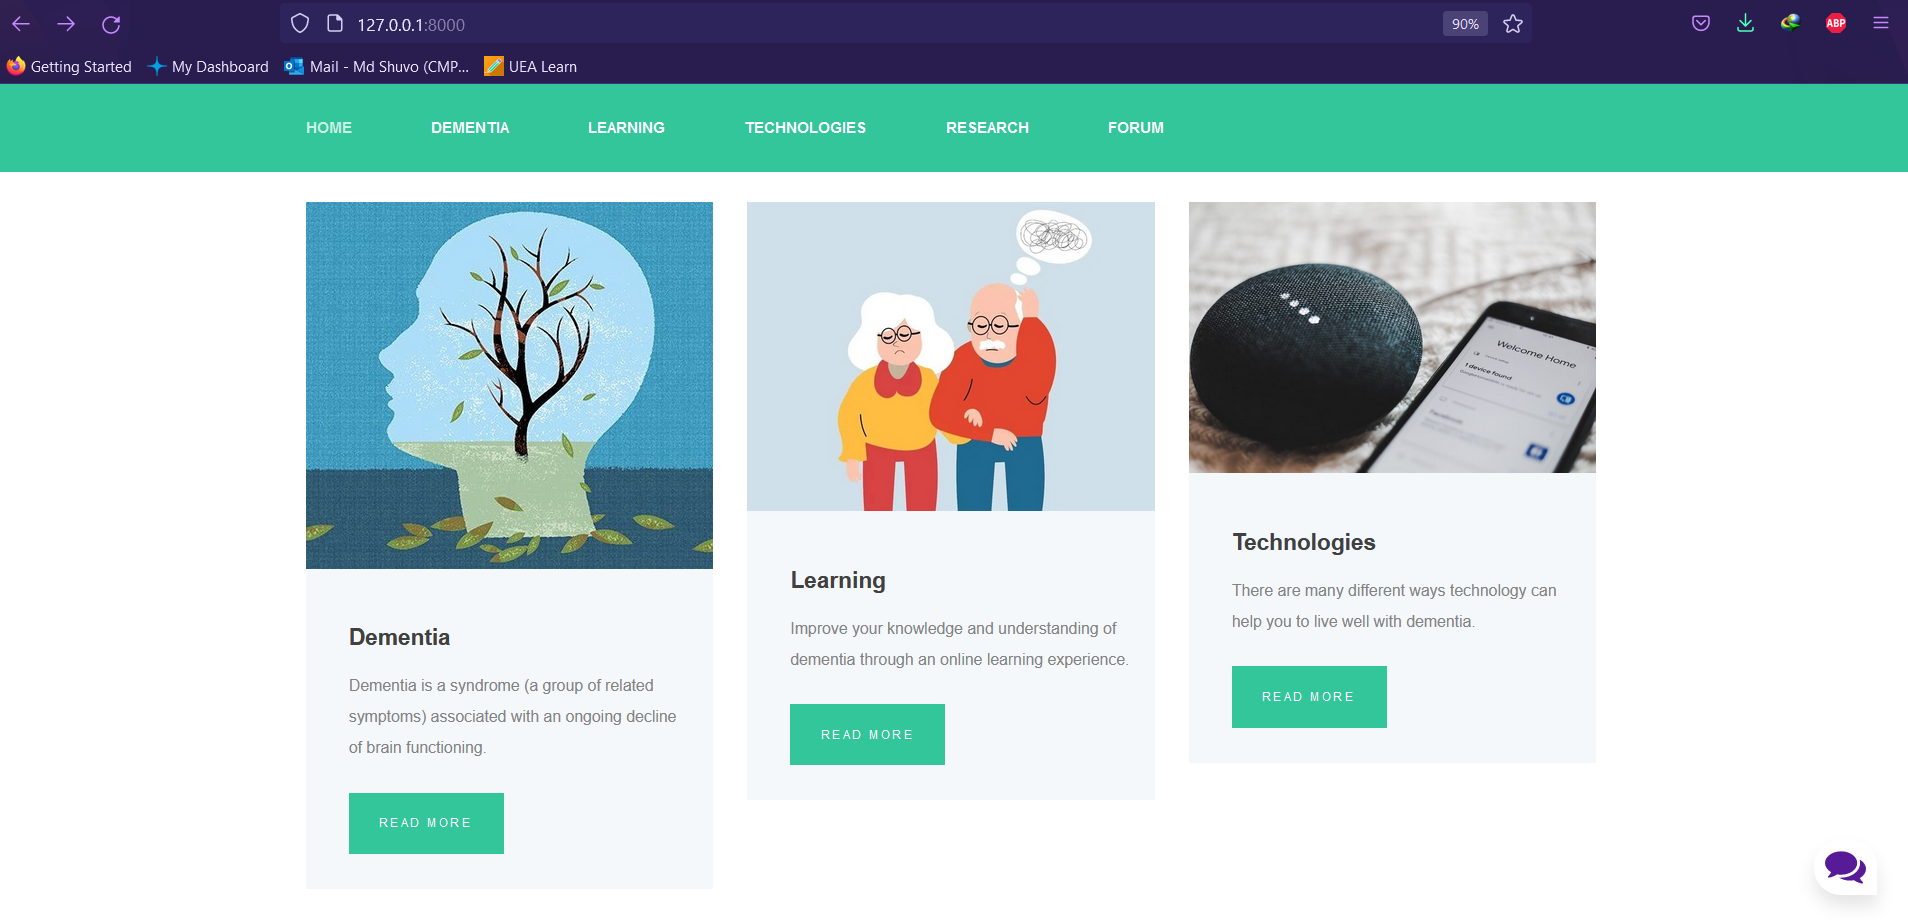
\includegraphics[width=0.85\textwidth]{home2}
	\caption{Homepage contains linked pages.}
	\label{fig:13}
\end{figure}

\begin{figure}[!h]
	\centering
	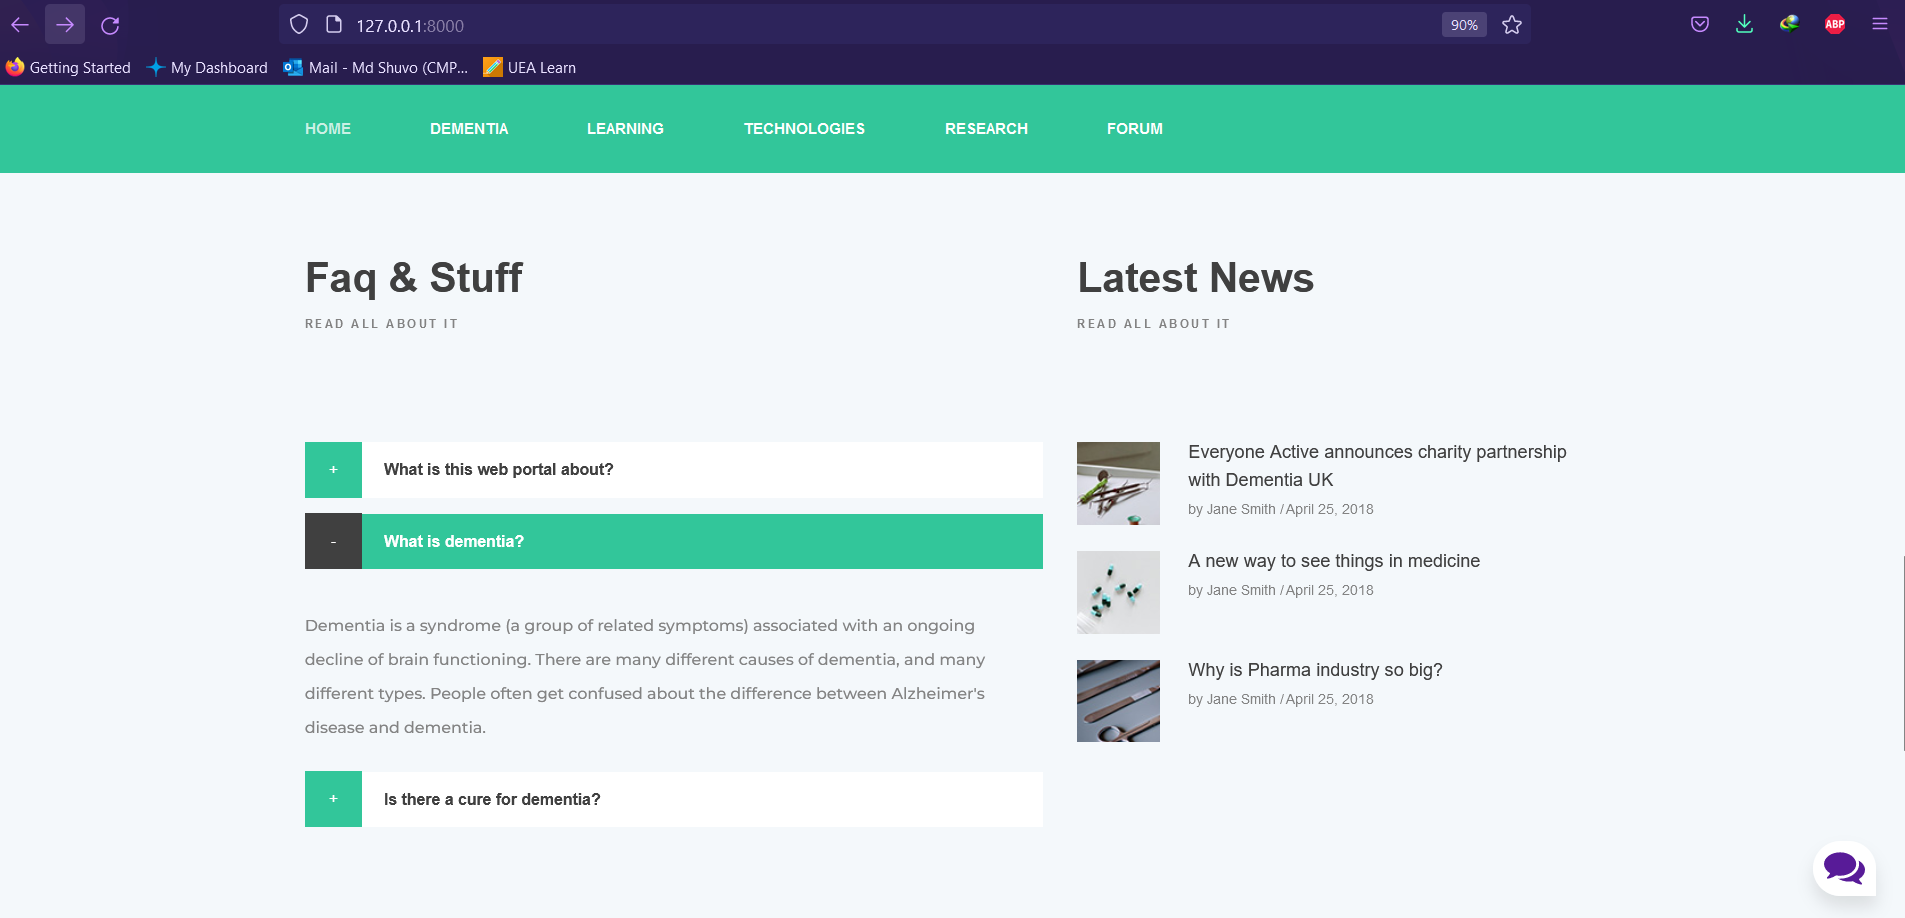
\includegraphics[width=0.85\textwidth]{home3}
	\caption{Homepage faq and recent articles.}
	\label{fig:14}
\end{figure}

\begin{figure}[!h]
	\centering
	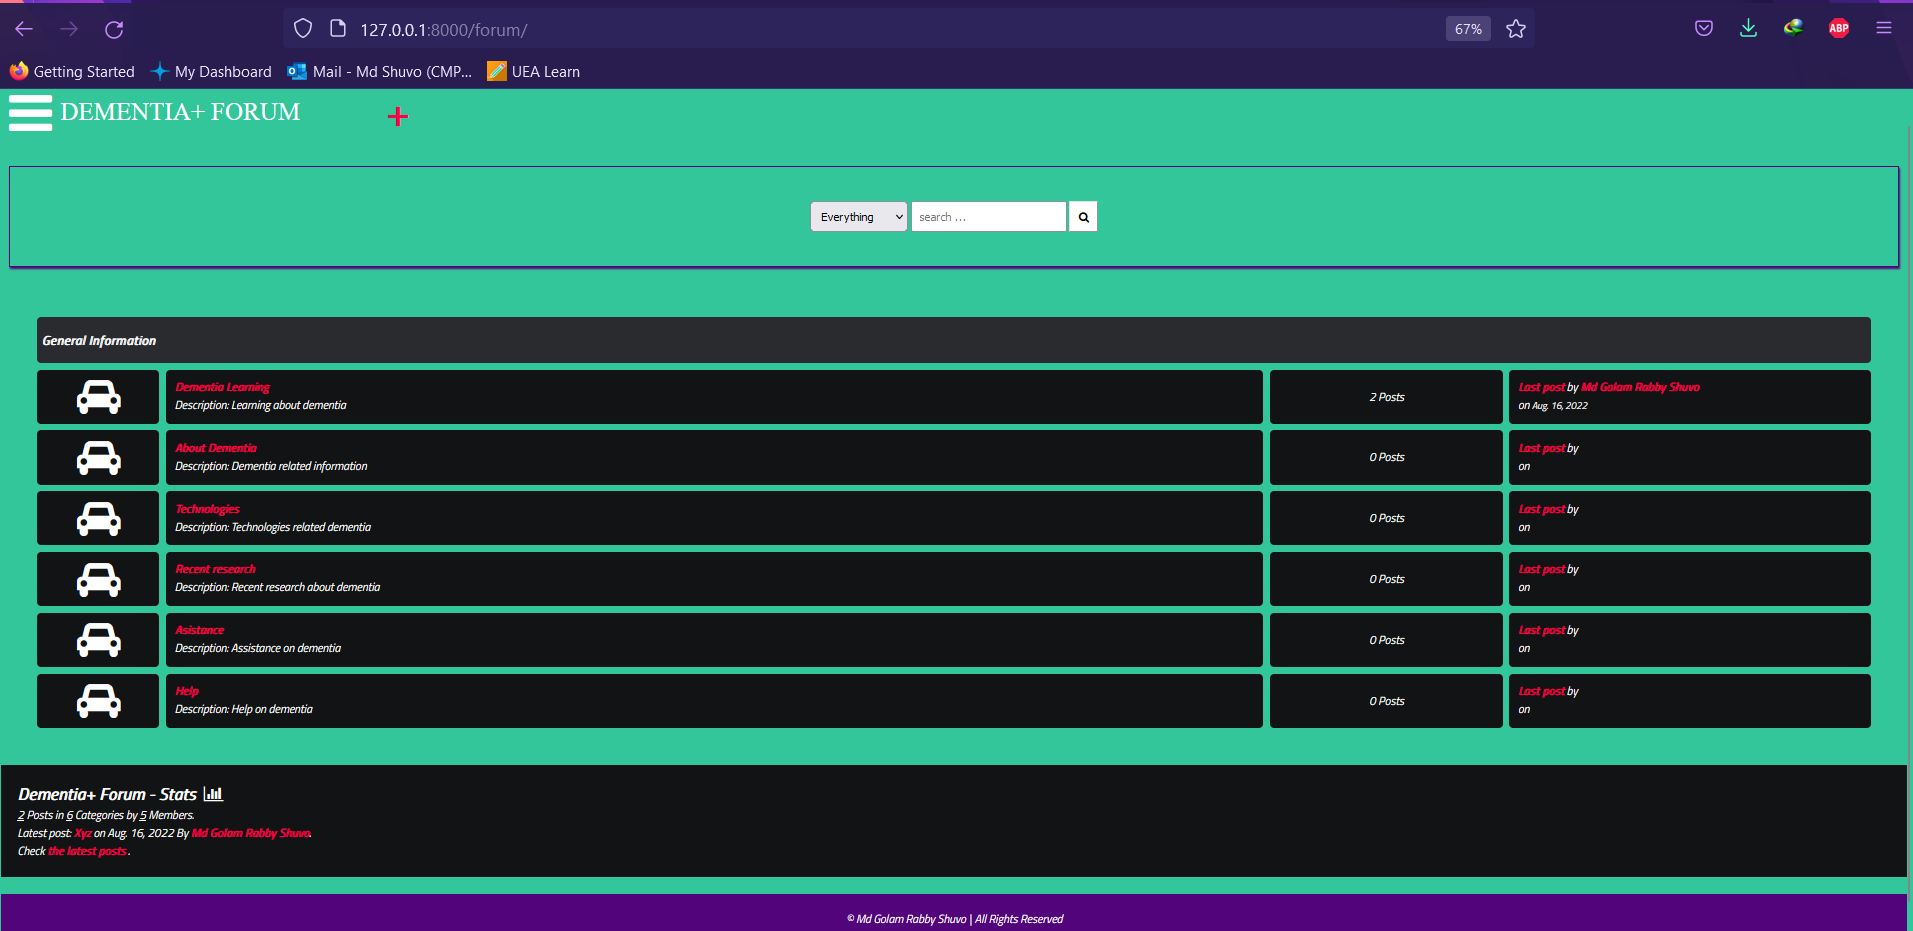
\includegraphics[width=0.85\textwidth]{forum}
	\caption{Forum homepage.}
	\label{fig:15}
\end{figure}

\begin{figure}[!h]
	\centering
	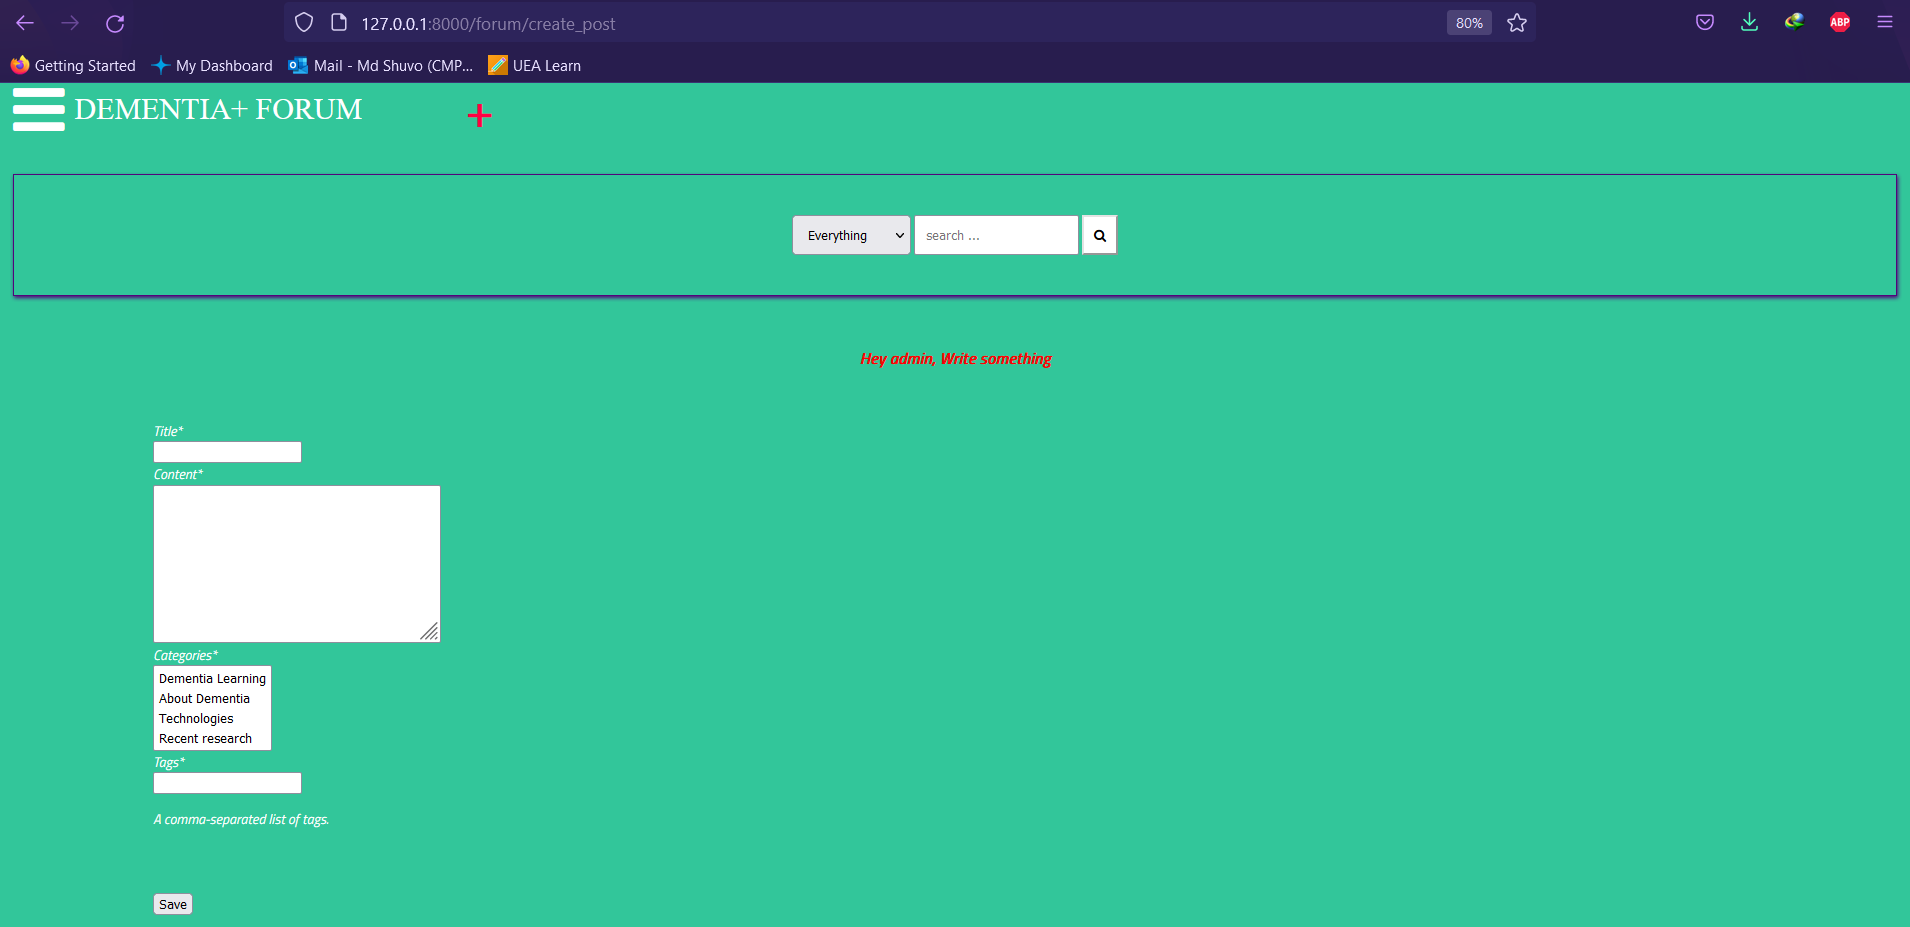
\includegraphics[width=0.85\textwidth]{create_post}
	\caption{Create post page.}
	\label{fig:16}
\end{figure}

\begin{figure}[!h]
	\centering
	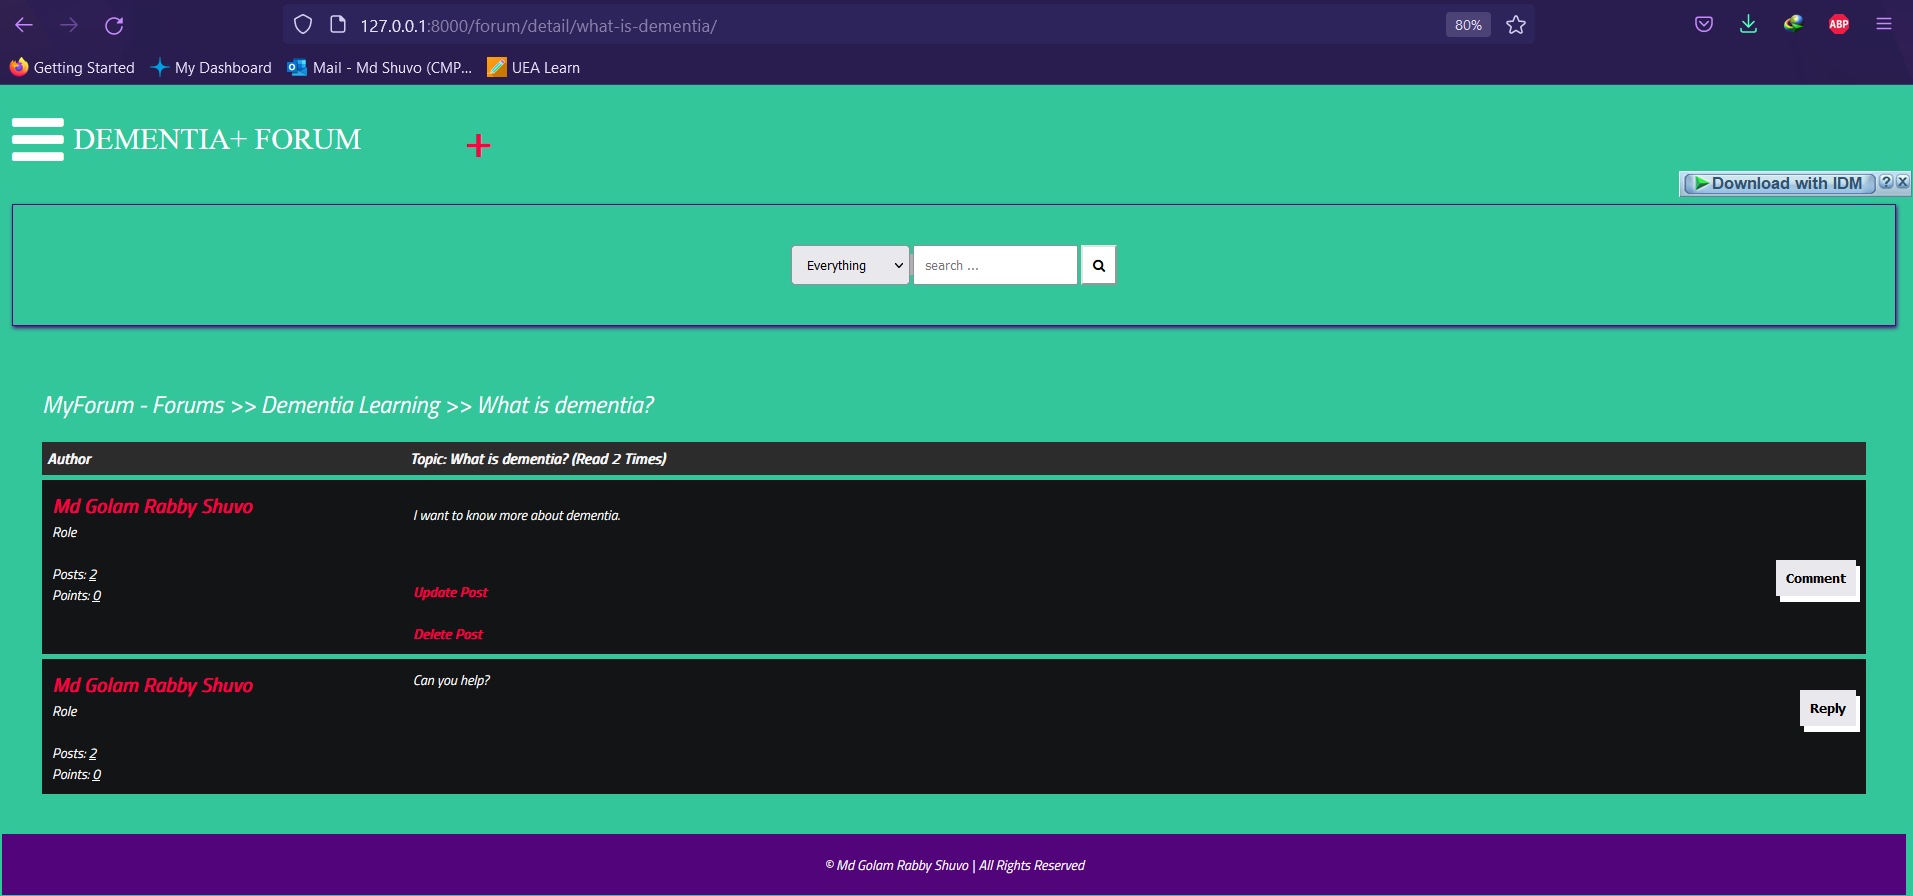
\includegraphics[width=0.85\textwidth]{post}
	\caption{A simple post.}
	\label{fig:17}
\end{figure}

\begin{figure}[!h]
	\centering
	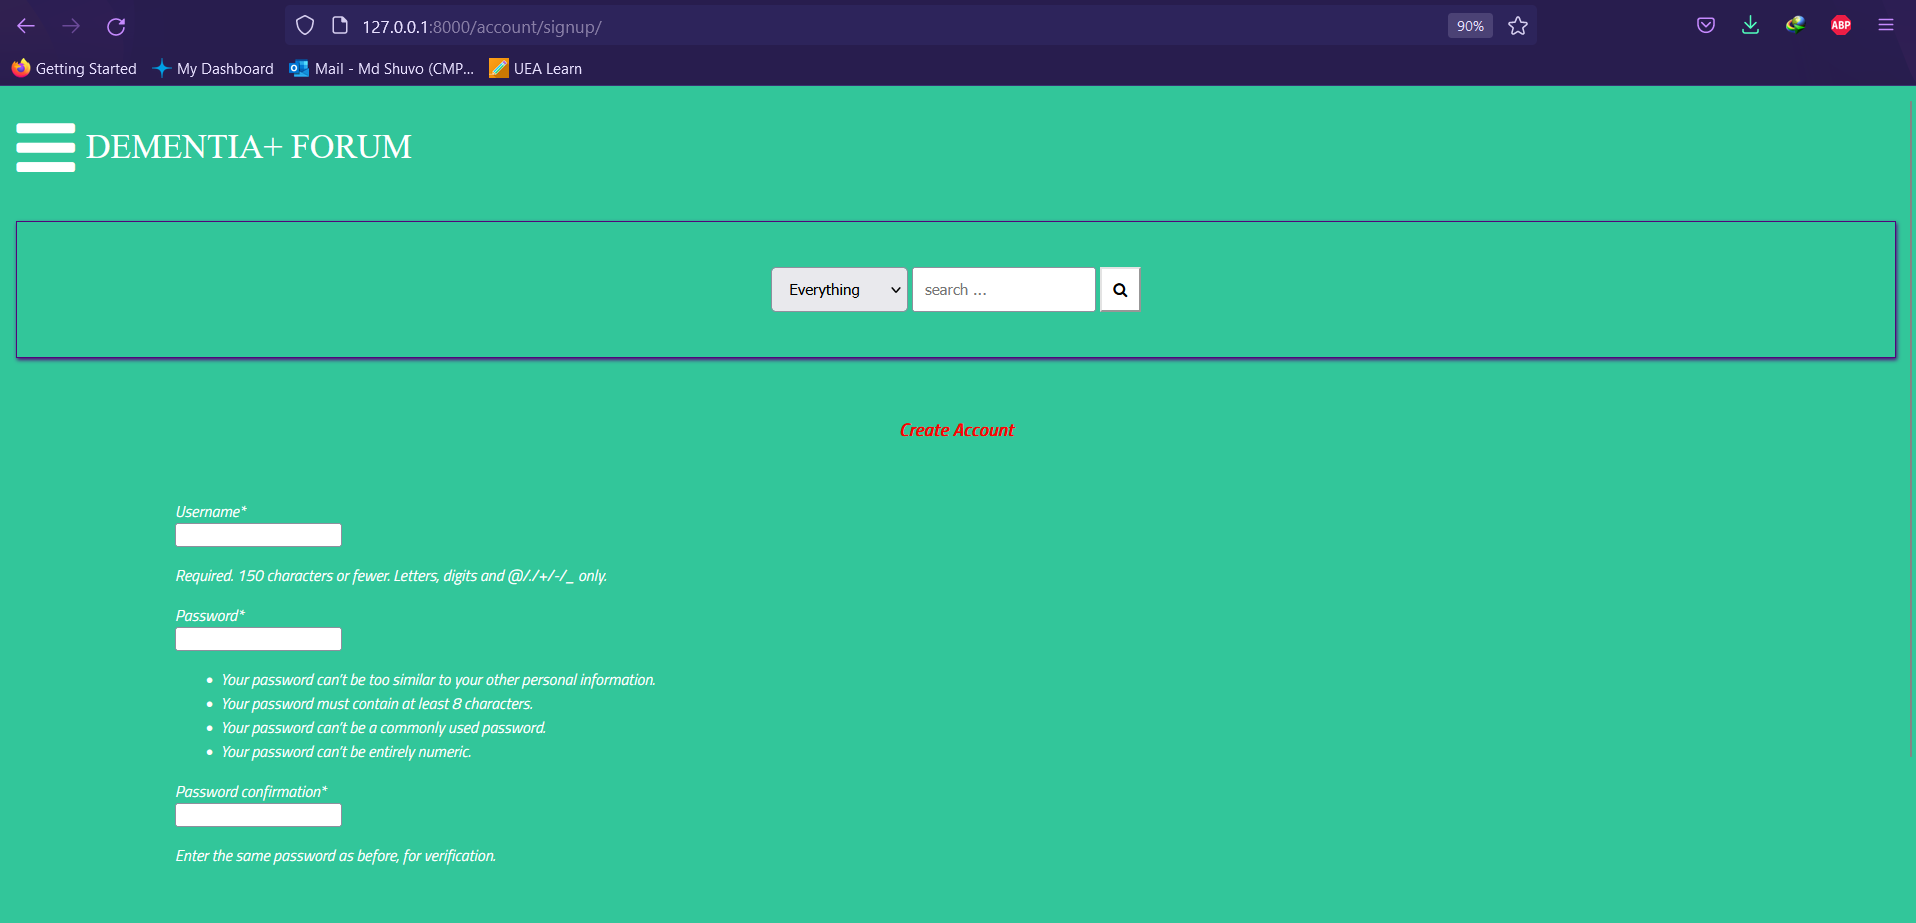
\includegraphics[width=0.85\textwidth]{signup}
	\caption{Signup page.}
	\label{fig:18}
\end{figure}

\begin{figure*}[ht!]
	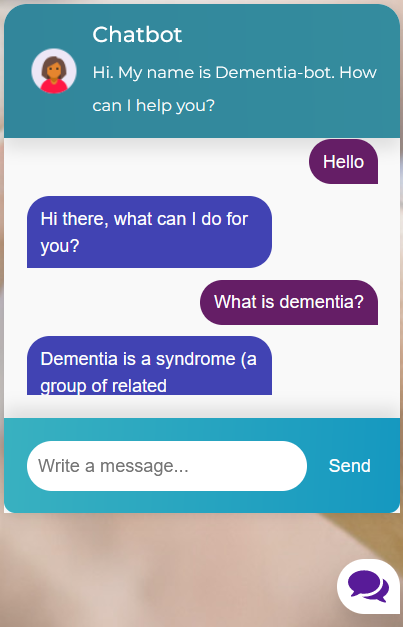
\includegraphics[width=.4\textwidth]{chat1}\hfill
	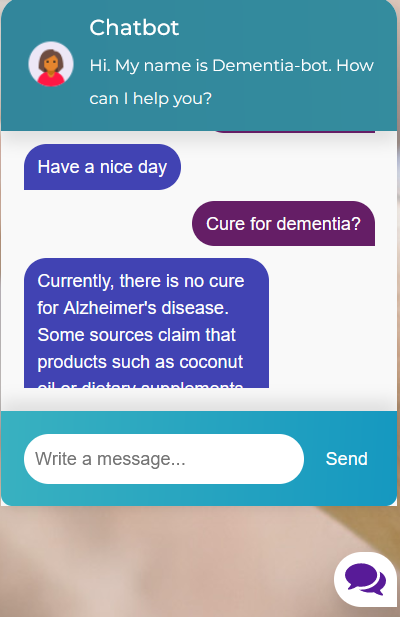
\includegraphics[width=.4\textwidth]{chat2}\hfill
	\caption{Chatbot in action.}
\end{figure*}

\def\baselinestretch{1.66}

%%% ----------------------------------------------------------------------
 

%%% ----------------------------------------------------------------------

